\documentclass[12pt,a4paper]{article}

\usepackage[UTF8]{ctex}
\usepackage{amsmath,amscd,amsbsy,amssymb,latexsym,url,bm,amsthm}
\usepackage{amsfonts}
\usepackage{epsfig,graphicx,subfigure}
\usepackage{hyperref}
\usepackage{listings}
\usepackage[vlined,ruled,linesnumbered]{algorithm2e}
\usepackage{enumitem}
\usepackage{xcolor}
\usepackage{geometry}

%\uppercase\expandafter{\romannumeral1}:% 罗马数字。

\lstset{
language=Matlab,
keywordstyle= \color{blue!70},
commentstyle= \color{red!50!green!50!blue!50},
breaklines
}%设置listing插入语言

\setlength{\parindent}{0em}
\setlength{\parskip}{1em}

\geometry{bottom =3cm}
\newcommand{\textbi}[1]{%
\textbf{\textit{#1}}}

\newcommand{\ncolor}[1]{%
{\color[RGB]{139,117,0}{#1}}}
\newtheorem{theorem}{Theorem}[section]
\newenvironment{solution}{{\noindent \it \textbf{Solution:}}\\}

\title{Evaluation model}
\author{Yunlong Cheng}

\begin{document}
\maketitle
\section{模型概念学习}
\href{run:../../7_14/cyl/LOG.pdf}{见此}。
\section{模型实例分析}
\subsection{层次分析法(AHP)}
\textbf{问题:}

假期某人想要出去旅游,现有三个目的地(方案):风光绮丽的杭州(P1)、迷人的北戴河(P2)和山水甲天下的桂林(P3)。假如选择的标准和依据(行动方案准则)有5个:景色,费用,饮食,居住和旅途。

\textbf{解答:}

\begin{enumerate}
  \item 
  \begin{center}
    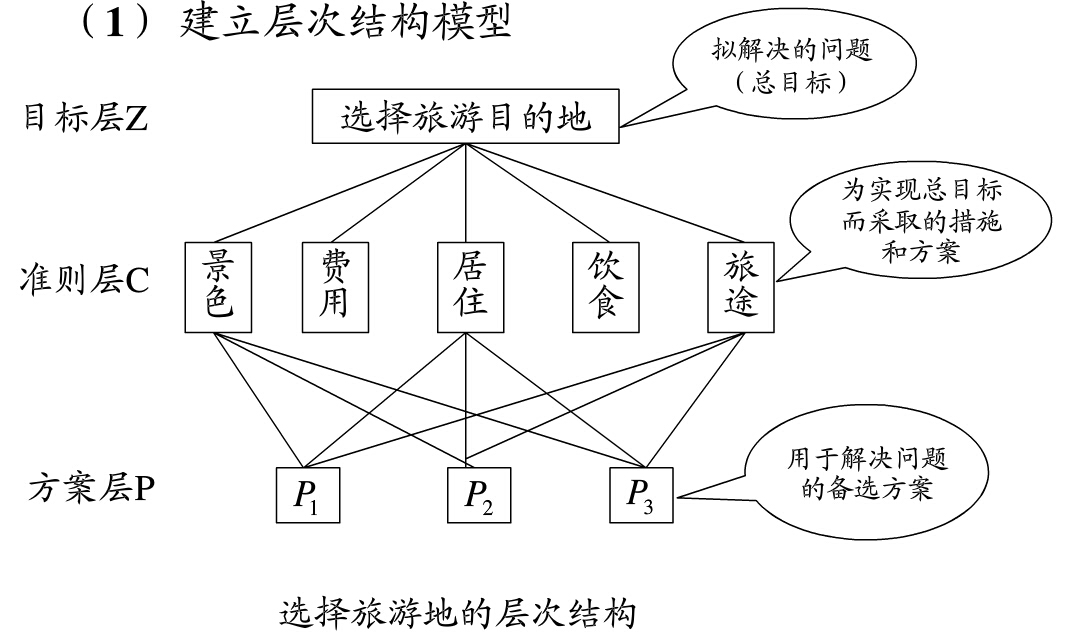
\includegraphics[width = \textwidth]{figures/structure.png}
  \end{center}
  \item 构造判断矩阵。
  \begin{figure}[!htbp]
    \centering
    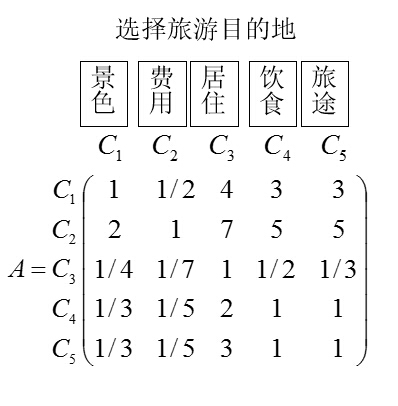
\includegraphics[width = 0.4\textwidth]{figures/target_criteria.png}
    \caption{目标-准则层判断矩阵(成对比较矩阵)}
  \end{figure}
  \\
  图二见下。
  \begin{figure}[!h]
    \centering
    \subfigure[方案-景色判断矩阵]{
      \begin{minipage}[t]{0.25\linewidth}
        \centering
        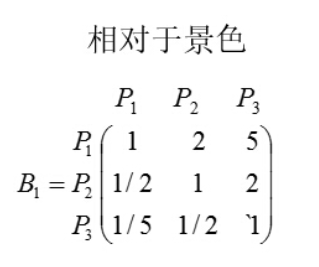
\includegraphics[width = 1in]{figures/plan_scene.png}
      \end{minipage}
    }
    \subfigure[方案-费用判断矩阵]{
      \begin{minipage}[t]{0.25\linewidth}
        \centering
        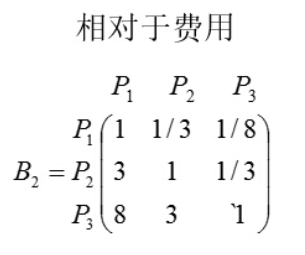
\includegraphics[width = 1in]{figures/plan_cost.png}
      \end{minipage}
    }
    \subfigure[方案-居住判断矩阵]{
      \begin{minipage}[t]{0.25\linewidth}
        \centering
        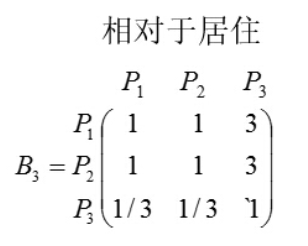
\includegraphics[width = 1in]{figures/plan_reside.png}
      \end{minipage}
    }
    \subfigure[方案-饮食判断矩阵]{
      \begin{minipage}[t]{0.25\linewidth}
        \centering
        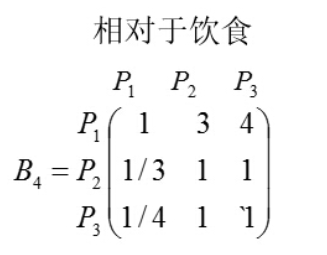
\includegraphics[width = 1in]{figures/plan_food.png}
      \end{minipage}
    }
    \subfigure[方案-旅途判断矩阵]{
      \begin{minipage}[t]{0.25\linewidth}
        \centering
        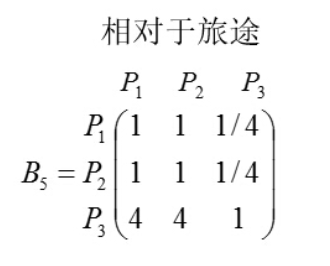
\includegraphics[width = 1in]{figures/plan_way.png}
      \end{minipage}
    }
    \caption{方案-准则层判断矩阵}
  \end{figure}
  \item 层次单排序:
  对上一层因素而言,本层次各因素的重要性的排序。

  计算方法:求矩阵 $A$ 的最大特征根与特征向量。
  其中 $\lambda_{max} = 5.073$ 对应的正规化特征向量为:
  $$\omega^{(2)} = (0.263,0.475,0.055,0.099,0.110)^T$$
  \item 一致性检验:
  $CI = \frac{\lambda_{max} - n}{n - 1} = \frac{5.073 - 5}{5 - 1} = 0.01825$

  查表知平均随机一致性指标 $RI$,则
  $$CR = \frac{CI}{RI} = \frac{0.01825}{1.12} = 0.016295 < 0.1$$
  检验通过。同理第二层一致性检验也通过。
  \item 得到的权重举证可以轻易结合到任何模型中去。
\end{enumerate}

\subsection{灰色关联分析与评价}
\textbf{问题:}

利用灰色关联分析对6位教师工作状况进行综合分析。

\textbf{解答:}
\begin{enumerate}
  \item 分析指标包括:专业素质、外语水平、教学工作量、科研成果、论文、著作与出勤。
  \item 对原始数据经处理后得到以下数值,见下表:
  \begin{center}
    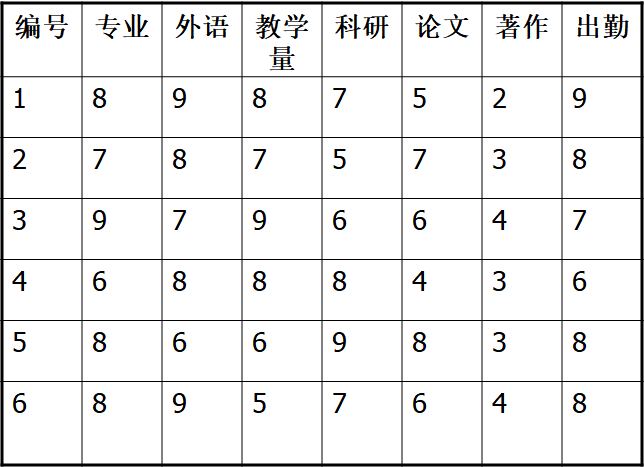
\includegraphics[width = 0.3\textwidth]{figures/2-data.png}
  \end{center}
  \item 确定参考序列:$\{x_0\} = \{9, 9, 9, 9, 8, 9, 9\}$
  \item 计算 $|x_0(k) - x_i(k)|$,见下表:
  \begin{center}
    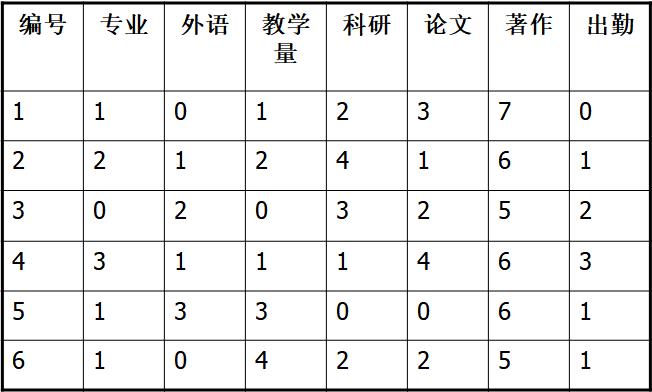
\includegraphics[width = 0.4\textwidth]{figures/2-less.png}
  \end{center}
  \item 求最值:
  $$\min_i\min_k|x_0(k) - x_i(k)| = \min(0,1,0,1,0,0) = 0$$
  $$\max_i\max_k|x_0(k) - x_i(k)| = \max(7,6,5,6,6,5) = 7$$
  \item 分辨系数 $\theta$ 取0.5,计算 $r_{ij}$,得:
  \begin{center}
    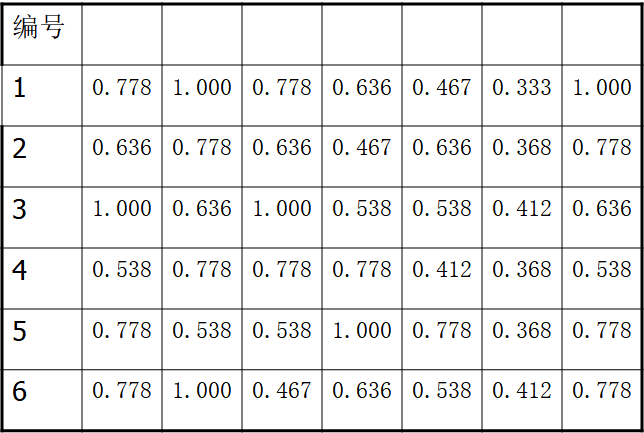
\includegraphics[width = 0.4\textwidth]{figures/rij.png}
  \end{center}
  \item 计算每个人的各指标关联系数的均值:
  $$r_{01} = \frac{0.778+1.000+0.778+0.636+0.467+0.333+1.000}{7} = 0.713$$
  $r_{02} = 0.614\quad r_{03} = 0.680\quad r_{04} = 0.599\quad r_{05} = 0.683\quad r_{06} = 0.658$。
  \item 考虑各指标权重,比较优劣。
\end{enumerate}
\end{document}
